\documentclass{book}
\usepackage[spanish]{babel}
\usepackage[T1]{fontenc}
\usepackage[utf8]{inputenc}
\usepackage{amsmath, amssymb}
\usepackage{dsfont}
\usepackage{graphics}
\usepackage{cases}
\usepackage{graphicx}
\usepackage{pgf}
\usepackage{epsfig}
\usepackage{amssymb}
\usepackage{multirow}
\usepackage{amstext}
\usepackage[ruled,vlined,lined]{algorithm2e}
\usepackage{listings}
\usepackage{amsmath}
\usepackage{epic}
\usepackage{epsfig}
\usepackage{fontenc}
\usepackage{framed,color}
\usepackage{palatino, url, multicol}

\begin{document}

\chapter{Procesamiento del Lenguaje Natural}

El volumen de datos textuales digitalizados que se genera cada día es enorme (por ejemplo, la web, redes sociales, registros médicos, libros digitalizados). Por lo tanto, también crece la necesidad de traducir, analizar y gestionar esta avalancha de palabras y texto.

El procesamiento del lenguaje natural (PLN) es el campo que se encarga de diseñar métodos y algoritmos que toman como entrada o producen como salida datos de \textbf{lenguaje natural} no estructurado \cite{goldberg2017neural}. El PLN se centra en el diseño y análisis de algoritmos computacionales y representaciones para procesar el lenguaje humano \cite{jacobbook}.

\section{Tareas de PLN}

Una tarea común de PLN es el Reconocimiento de Entidades Nombradas (NER, por sus siglas en inglés). Por ejemplo:

\begin{figure}[h]
	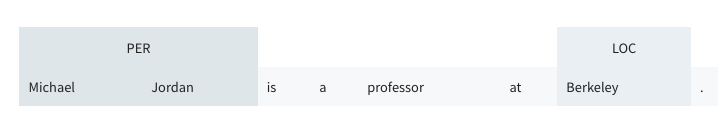
\includegraphics[scale=0.4]{pics/NER.png}
	\caption{Reconocimiento de Entidades Nombradas}
\end{figure}

El lenguaje humano es altamente ambiguo, como en las frases: "Comí pizza con amigos", "Comí pizza con aceitunas" o "Comí pizza con un tenedor". Además, el lenguaje está en constante cambio y evolución, como ocurre con los hashtags en Twitter.

\section{PLN y Lingüística Computacional}

El procesamiento del lenguaje natural (PLN) desarrolla métodos para resolver problemas prácticos relacionados con el lenguaje \cite{JohnsonMLSS}.

Algunos ejemplos son:

\begin{itemize}
  \item Reconocimiento automático del habla.
  \item Traducción automática.
  \item Extracción de información de documentos.
\end{itemize}

La lingüística computacional (LC) estudia los procesos computacionales subyacentes al lenguaje (humano).

\begin{itemize}
  \item ¿Cómo comprendemos el lenguaje?
  \item ¿Cómo producimos el lenguaje?
  \item ¿Cómo aprendemos el lenguaje?
\end{itemize}

El PLN y la LC utilizan métodos y modelos similares.

\section{Diferencia entre PLN y LC}

Aunque existe una superposición sustancial, hay una diferencia importante en el enfoque. La LC se centra en la lingüística respaldada por métodos computacionales (similar a la biología computacional o la astronomía computacional). En lingüística, el lenguaje es el objeto de estudio. El PLN se centra en resolver tareas bien definidas relacionadas con el lenguaje humano (como la traducción, la respuesta a consultas, las conversaciones). Si bien los conocimientos lingüísticos fundamentales pueden ser cruciales para realizar estas tareas, el éxito se mide en función de si y cómo se logra el objetivo (según una métrica de evaluación) \cite{jacobbook}.



El procesamiento del lenguaje natural y la lingüística computacional están estrechamente relacionados y se superponen en muchos aspectos. Ambos campos utilizan métodos y modelos similares para abordar problemas relacionados con el lenguaje humano. Sin embargo, la diferencia principal radica en el enfoque: la lingüística computacional se centra en la lingüística respaldada por métodos computacionales, mientras que el procesamiento del lenguaje natural se centra en resolver tareas prácticas relacionadas con el lenguaje. Ambos campos son fundamentales para comprender y aprovechar el poder del lenguaje humano en la era digital.


\section{Niveles de descripción lingüística}

El campo de la \textbf{descripción lingüística} abarca diferentes niveles:

\begin{itemize}
  \item \textbf{Fonética y fonología:} estudio de los sonidos del habla.
  \item \textbf{Morfología:} estudio de la estructura de las palabras.
  \item \textbf{Sintaxis:} estudio de la estructura de las oraciones.
  \item \textbf{Semántica:} estudio del significado de las palabras y oraciones.
  \item \textbf{Pragmática:} estudio del uso del lenguaje en el contexto.
\end{itemize}

El PLN puede abordar tareas en cada uno de estos niveles, pero a menudo se enfoca en niveles más altos de representación y comprensión.




\section{Fonética}

La fonética es la rama de la lingüística que se ocupa del estudio de los sonidos del lenguaje. Examina los órganos utilizados en la producción de sonidos, como la boca, la lengua, la garganta, la nariz, los labios y el paladar. Los sonidos del lenguaje se dividen en vocales y consonantes. Las vocales se producen con poca restricción del flujo de aire desde los pulmones, mientras que las consonantes implican alguna restricción o cierre en el tracto vocal \cite{JohnsonMLSS, fromkin2018introduction}. Además, el Alfabeto Fonético Internacional (AFI) proporciona una notación alfabética para representar los sonidos fonéticos.

\section{Fonología}

La fonología se centra en el estudio de cómo los sonidos del habla forman patrones y construyen significado. Los fonemas son las unidades básicas de sonido que diferencian el significado de las palabras. Por ejemplo, en inglés, la "p" y la "b" son fonemas distintos porque cambian el significado de las palabras en las que se encuentran. La fonología también examina las variaciones en la pronunciación de los sonidos en diferentes contextos y dialectos \cite{fromkin2018introduction}.

\section{Morfología}

La morfología se ocupa del estudio de la estructura interna de las palabras. Los morfemas son las unidades mínimas de significado que componen las palabras. Por ejemplo, en la palabra "deshacer", los morfemas son "des-", "hacer" y "-er". La morfología también se interesa por los procesos de formación de palabras, como la derivación, donde se agregan prefijos o sufijos a una palabra existente para formar una nueva palabra con un significado diferente \cite{JohnsonMLSS}.

\section{Sintaxis}

La sintaxis es el estudio de cómo las palabras se combinan para formar frases y oraciones gramaticales. Examina las reglas y estructuras que determinan la organización de las palabras en una oración y cómo influyen en el significado. La sintaxis también se ocupa de la relación entre las palabras y las funciones que desempeñan dentro de una oración. Por ejemplo, en la oración "El perro persigue al gato", "el perro" es el sujeto, "persigue" es el verbo y "al gato" es el complemento directo \cite{JohnsonMLSS}.

\section{Semántica}

La semántica es el estudio del significado de las palabras, las frases y las oraciones. Examina cómo se construye y se interpreta el significado en el contexto del lenguaje. La semántica también se interesa por los roles semánticos, que indican la función de cada entidad en una oración. Por ejemplo, en la oración "El niño cortó la cuerda con una navaja", "el niño" es el agente, "la cuerda" es el tema y "una navaja" es el instrumento \cite{JohnsonMLSS}.

\section{Pragmática}

La pragmática se centra en cómo el contexto influye en la interpretación y el significado de las expresiones lingüísticas. Examina cómo se utilizan las expresiones lingüísticas en situaciones reales y cómo los hablantes interpretan el significado implícito. Por ejemplo, la oración "Hace frío aquí" puede interpretarse como una sugerencia implícita de cerrar las ventanas \cite{fromkin2018introduction}.


\section{Procesamiento del Lenguaje Natural y Aprendizaje Automático}

Aunque los seres humanos somos grandes usuarios del lenguaje, también somos muy malos para comprender y describir formalmente las reglas que rigen el lenguaje.

Entender y producir lenguaje utilizando computadoras es altamente desafiante. Los métodos más conocidos para lidiar con datos de lenguaje se basan en el aprendizaje automático supervisado.

El aprendizaje automático supervisado consiste en intentar inferir patrones y regularidades a partir de un conjunto de pares de entrada y salida preanotados (también conocido como conjunto de datos de entrenamiento).

\section{Conjunto de Datos de Entrenamiento: Datos de NER CoNLL-2003}

Cada línea contiene un token, una etiqueta de parte de la oración, una etiqueta de sintagma y una etiqueta de entidad nombrada.
\begin{center}
\begin{verbatim}
U.N.         NNP  I-NP  I-ORG
official     NN   I-NP  O
Ekeus        NNP  I-NP  I-PER
heads        VBZ  I-VP  O
for          IN   I-PP  O
Baghdad      NNP  I-NP  I-LOC
.            .    O     O
\end{verbatim}
\end{center}

\footnotemark{Fuente: \url{https://www.clips.uantwerpen.be/conll2003/ner/}}

\section{Desafíos del Lenguaje}

Existen tres propiedades desafiantes del lenguaje: la discreción, la composicionalidad y la dispersión.

\textbf{Discreción}: no podemos inferir la relación entre dos palabras a partir de las letras que las componen (por ejemplo, hamburguesa y pizza).

\textbf{Composicionalidad}: el significado de una oración va más allá del significado individual de sus palabras.

\textbf{Dispersión}: la forma en que las palabras (símbolos discretos) pueden combinarse para formar significados es prácticamente infinita.



\section{Ejemplo de tareas NLP}

\paragraph{Clasificación de temas}
La clasificación por temas es una tarea de PLN en la que un documento se clasifica en una de varias categorías, como deportes, política, cotilleos o economía. Las palabras de los documentos proporcionan pistas importantes sobre su tema. Sin embargo, escribir reglas para esta tarea es un reto debido a la complejidad del lenguaje. La anotación de datos, en la que los lectores clasifican los documentos por temas, puede ayudar a crear datos de entrenamiento para algoritmos de aprendizaje automático supervisado. Estos algoritmos aprenden patrones de uso de palabras que ayudan en la categorización de documentos.

\paragraph{Análisis de Sentimiento}
El análisis de sentimientos es la aplicación de técnicas de PLN para identificar y extraer información subjetiva de conjuntos de datos textuales. Un problema común en el análisis de sentimientos es la clasificación de la polaridad a nivel de mensaje (MPC), en la que las frases se clasifican automáticamente como positivas, negativas o neutras. Las soluciones más avanzadas utilizan modelos de aprendizaje automático supervisado entrenados con ejemplos anotados manualmente.

En la clasificación de sentimientos, se suele utilizar el aprendizaje supervisado, siendo las máquinas de vectores de soporte (SVM) una opción popular. El objetivo de las SVM es encontrar un hiperplano que separe las clases con el máximo margen, logrando la mejor separación entre clases positivas, negativas y neutras \cite{jacobbook}.

El conocimiento de las estructuras lingüísticas es importante para el diseño de características y el análisis de errores en PNL. Los enfoques de aprendizaje automático en PNL se basan en características que describen y generalizan las instancias de uso del lenguaje. Los conocimientos lingüísticos guían la selección y el diseño de los rasgos, ayudando al algoritmo de aprendizaje automático a encontrar correlaciones entre el uso de la lengua y las etiquetas de destino \cite{bender2013linguistic}.

La PNL plantea varios retos, como los costes de anotación, las variaciones de dominio y la necesidad de actualizaciones continuas. La anotación manual requiere mucho trabajo y tiempo. Las variaciones de dominio exigen el aprendizaje de patrones diferentes para los distintos corpus. Los modelos entrenados en un dominio pueden no funcionar bien en otro. Además, los modelos de PNL pueden quedar obsoletos a medida que el uso del lenguaje evoluciona con el tiempo.








En este capítulo, hemos explorado el desafío de entender y producir lenguaje utilizando computadoras. El aprendizaje automático supervisado es una de las principales técnicas utilizadas para abordar este desafío. Además, hemos discutido las propiedades desafiantes del lenguaje, como la discreción, la composicionalidad y la dispersión. Estos aspectos nos muestran la complejidad inherente al procesamiento del lenguaje natural y nos desafían a encontrar soluciones efectivas.



\bibliography{bio}
\bibliographystyle{apalike}

\end{document}
